%-*-latex-*-
\sectionthree{Heap and complete trees}
\begin{python0}
from solutions import *; clear()
\end{python0}

Recall that we have complete freedom in choosing where to insert a new node.
We also have complete freedom in choosing any leaf to use to overwrite
a node to be deleted as long as the leaf is a descendent of the node whose
value is to delete.
In particular, if we are remove the value of the root of the heap,
we can choose any leaf.

It's because of the above,
after every insert and root value removal,
we can alway ensure that the heap is complete.
Recall that a complete binary tree that is almost full except that the
last level might not have all the leaves.
are at the same level.
Furthermore, we can force to have
all the leaves to be all on the left side of the whole
tree.
This is what I mean by \lq\lq left side'' of the tree:

\begin{center}
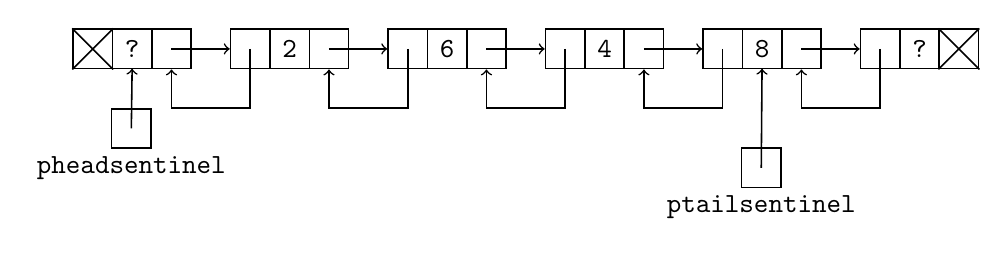
\begin{tikzpicture}

\draw (0.25, 0.25)
  node[draw, line width=0.02cm, , color=black,
       rounded corners=0cm, inner sep=0cm] {

\begin{minipage}[t][0.5cm]{0.5cm}
\mbox{}

\end{minipage}

};\draw (0.25, 0.25) node[color=black] {{\texttt{}}};
\draw (0.75, 0.25)
  node[draw, line width=0.02cm, , color=black,
       rounded corners=0cm, inner sep=0cm] {

\begin{minipage}[t][0.5cm]{0.5cm}
\mbox{}

\end{minipage}

};\draw (0.75, 0.25) node[color=black] {{\texttt{?}}};
\draw (1.25, 0.25)
  node[draw, line width=0.02cm, , color=black,
       rounded corners=0cm, inner sep=0cm] {

\begin{minipage}[t][0.5cm]{0.5cm}
\mbox{}

\end{minipage}

};\draw (1.25, 0.25) node[color=black] {{\texttt{}}};
\draw (2.25, 0.25)
  node[draw, line width=0.02cm, , color=black,
       rounded corners=0cm, inner sep=0cm] {

\begin{minipage}[t][0.5cm]{0.5cm}
\mbox{}

\end{minipage}

};\draw (2.25, 0.25) node[color=black] {{\texttt{}}};
\draw (2.75, 0.25)
  node[draw, line width=0.02cm, , color=black,
       rounded corners=0cm, inner sep=0cm] {

\begin{minipage}[t][0.5cm]{0.5cm}
\mbox{}

\end{minipage}

};\draw (2.75, 0.25) node[color=black] {{\texttt{2}}};
\draw (3.25, 0.25)
  node[draw, line width=0.02cm, , color=black,
       rounded corners=0cm, inner sep=0cm] {

\begin{minipage}[t][0.5cm]{0.5cm}
\mbox{}

\end{minipage}

};\draw (3.25, 0.25) node[color=black] {{\texttt{}}};
\draw (4.25, 0.25)
  node[draw, line width=0.02cm, , color=black,
       rounded corners=0cm, inner sep=0cm] {

\begin{minipage}[t][0.5cm]{0.5cm}
\mbox{}

\end{minipage}

};\draw (4.25, 0.25) node[color=black] {{\texttt{}}};
\draw (4.75, 0.25)
  node[draw, line width=0.02cm, , color=black,
       rounded corners=0cm, inner sep=0cm] {

\begin{minipage}[t][0.5cm]{0.5cm}
\mbox{}

\end{minipage}

};\draw (4.75, 0.25) node[color=black] {{\texttt{6}}};
\draw (5.25, 0.25)
  node[draw, line width=0.02cm, , color=black,
       rounded corners=0cm, inner sep=0cm] {

\begin{minipage}[t][0.5cm]{0.5cm}
\mbox{}

\end{minipage}

};\draw (5.25, 0.25) node[color=black] {{\texttt{}}};
\draw (6.25, 0.25)
  node[draw, line width=0.02cm, , color=black,
       rounded corners=0cm, inner sep=0cm] {

\begin{minipage}[t][0.5cm]{0.5cm}
\mbox{}

\end{minipage}

};\draw (6.25, 0.25) node[color=black] {{\texttt{}}};
\draw (6.75, 0.25)
  node[draw, line width=0.02cm, , color=black,
       rounded corners=0cm, inner sep=0cm] {

\begin{minipage}[t][0.5cm]{0.5cm}
\mbox{}

\end{minipage}

};\draw (6.75, 0.25) node[color=black] {{\texttt{4}}};
\draw (7.25, 0.25)
  node[draw, line width=0.02cm, , color=black,
       rounded corners=0cm, inner sep=0cm] {

\begin{minipage}[t][0.5cm]{0.5cm}
\mbox{}

\end{minipage}

};\draw (7.25, 0.25) node[color=black] {{\texttt{}}};
\draw (8.25, 0.25)
  node[draw, line width=0.02cm, , color=black,
       rounded corners=0cm, inner sep=0cm] {

\begin{minipage}[t][0.5cm]{0.5cm}
\mbox{}

\end{minipage}

};\draw (8.25, 0.25) node[color=black] {{\texttt{}}};
\draw (8.75, 0.25)
  node[draw, line width=0.02cm, , color=black,
       rounded corners=0cm, inner sep=0cm] {

\begin{minipage}[t][0.5cm]{0.5cm}
\mbox{}

\end{minipage}

};\draw (8.75, 0.25) node[color=black] {{\texttt{8}}};
\draw (9.25, 0.25)
  node[draw, line width=0.02cm, , color=black,
       rounded corners=0cm, inner sep=0cm] {

\begin{minipage}[t][0.5cm]{0.5cm}
\mbox{}

\end{minipage}

};\draw (9.25, 0.25) node[color=black] {{\texttt{}}};
\draw (10.25, 0.25)
  node[draw, line width=0.02cm, , color=black,
       rounded corners=0cm, inner sep=0cm] {

\begin{minipage}[t][0.5cm]{0.5cm}
\mbox{}

\end{minipage}

};\draw (10.25, 0.25) node[color=black] {{\texttt{}}};
\draw (10.75, 0.25)
  node[draw, line width=0.02cm, , color=black,
       rounded corners=0cm, inner sep=0cm] {

\begin{minipage}[t][0.5cm]{0.5cm}
\mbox{}

\end{minipage}

};\draw (10.75, 0.25) node[color=black] {{\texttt{?}}};
\draw (11.25, 0.25)
  node[draw, line width=0.02cm, , color=black,
       rounded corners=0cm, inner sep=0cm] {

\begin{minipage}[t][0.5cm]{0.5cm}
\mbox{}

\end{minipage}

};\draw (11.25, 0.25) node[color=black] {{\texttt{}}};\draw[line width=0.02cm,black,->] (1.25,0.25) to  (1.99,0.25);
\draw[line width=0.02cm,black,->] (3.25,0.25) to  (3.99,0.25);
\draw[line width=0.02cm,black,->] (2.25,0.25) to  (2.25,-0.5) to  (1.25,-0.5) to  (1.25,-0.01);
\draw[line width=0.02cm,black,->] (5.25,0.25) to  (5.99,0.25);
\draw[line width=0.02cm,black,->] (4.25,0.25) to  (4.25,-0.5) to  (3.25,-0.5) to  (3.25,-0.01);
\draw[line width=0.02cm,black,->] (7.25,0.25) to  (7.99,0.25);
\draw[line width=0.02cm,black,->] (6.25,0.25) to  (6.25,-0.5) to  (5.25,-0.5) to  (5.25,-0.01);
\draw[line width=0.02cm,black,->] (9.25,0.25) to  (9.99,0.25);
\draw[line width=0.02cm,black,->] (8.25,0.25) to  (8.25,-0.5) to  (7.25,-0.5) to  (7.25,-0.01);
\draw[line width=0.02cm,black,->] (10.25,0.25) to  (10.25,-0.5) to  (9.25,-0.5) to  (9.25,-0.01);
\draw[line width=0.02cm,black] (-0.01,0.51) to  (0.51,-0.01);
\draw[line width=0.02cm,black] (0.51,0.51) to  (-0.01,-0.01);
\draw[line width=0.02cm,black] (10.99,0.51) to  (11.51,-0.01);
\draw[line width=0.02cm,black] (11.51,0.51) to  (10.99,-0.01);

\draw (0.74, -0.76)
  node[draw, line width=0.02cm, , color=black,
       rounded corners=0cm, inner sep=0cm] {

\begin{minipage}[t][0.5cm]{0.5cm}
\mbox{}

\end{minipage}

};\draw (0.74, -0.76) node[color=black] {{\texttt{}}};
\draw (0.74, -1.26)
  node[draw, line width=0.02cm, , color=white,
       rounded corners=0cm, inner sep=0cm] {

\begin{minipage}[t][0.1cm]{0.1cm}
\mbox{}

\end{minipage}

};\draw (0.74, -1.26) node[color=black] {{\texttt{pheadsentinel}}};\draw[line width=0.02cm,black,->] (0.74,-0.76) to  (0.75,0);

\draw (8.74, -1.26)
  node[draw, line width=0.02cm, , color=black,
       rounded corners=0cm, inner sep=0cm] {

\begin{minipage}[t][0.5cm]{0.5cm}
\mbox{}

\end{minipage}

};\draw (8.74, -1.26) node[color=black] {{\texttt{}}};
\draw (8.74, -1.76)
  node[draw, line width=0.02cm, , color=white,
       rounded corners=0cm, inner sep=0cm] {

\begin{minipage}[t][0.1cm]{0.1cm}
\mbox{}

\end{minipage}

};\draw (8.74, -1.76) node[color=black] {{\texttt{ptailsentinel}}};\draw[line width=0.02cm,black,->] (8.74,-1.26) to  (8.75,0);
\end{tikzpicture}

\end{center}



This can be achieved by
\begin{tightlist}
\li During insert, always insert a leaf just to the right of the
rightmost leaf at the last level.
\li During delete, always using the right most leaf of the 
last level whenever we remove the root.
\end{tightlist}




\newpage
\begin{ex}
Build a maxheap by inserting the following into an empty tree:
1, 3, 5, 7, 6, 4, 2, 8, 9, 0.
Make sure the tree is complete after each insert and the leaves
at the lowest level are all on the left.
\qed
\end{ex}

\newpage
\begin{ex}
Using the maxheap from the previous question,
remove the following values one after another:
1, 3, 5, 7, 6, 4, 2, 8, 9, 0.
Make sure that after each delete, the tree is complete after each insert and the leaves
at the lowest level are all on the left.
\qed
\end{ex}

\newpage
\begin{ex}
  Suppose that in maxheap, there are two 5's.
  One 5 was inserted at 9AM and the second 5 was inserted
  at 10AM.
  If I delete the maximum value of the heap
  until the heap is empty,
  will the 5 inserted at 9AM be deleted
  from the heap
  before or after the 5 inserted at 10AM?
  Or are both scenarios possible?
\end{ex}

\newpage
Being complete means that the heaps can have the minimal possible height.
At this point, you ought to know that this is a good thing.

This also implies right away that the worse runtimes for 
insert and delete is $O(\log n)$ for both insert and delete
as long as we keep the heap complete.

